\chapter{Diamond}
To start with investigated regular $3D$ diamond crystal. I considered here the case where we have only one set of $s$, $p_z$, $p_y$, and $p_z$ orbitals at each
atomic site (used parameters are placed at the table \ref{tab:diamond_params}). Calculated band structure is placed on the fig. \ref{fig:tb_diamond}. Agreemnet with experimantal results (fig. \ref{fig:theory_diamond}) is quite good.
\begin{figure}[h] 
 \begin{center}
  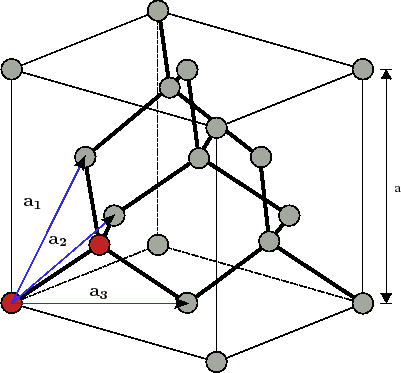
\includegraphics[width=0.3\linewidth]{img/diamond_crystall}
  \caption{Diamond crystall structure.}
 \end{center}
\end{figure}

\begin{table}[h]
 \begin{center}
  \begin{tabular}{|c|c|}
  \hline
    Parameter&Value, [eV]\\ \hline
    $\epsilon_s$ & $0.0$ \\ \hline
    $\epsilon_p$ & $7.4$ \\ \hline
    $V_{ss \sigma}$ & $-3.8$  \\ \hline
    $V_{sp \sigma}$ & $4.44$\\ \hline
    $V_{pp \sigma}$ & $-1.325$ \\ \hline
    $V_{pp \pi}$ &  $4.9$\\ \hline
  \end{tabular}
 \end{center}
  \caption{TB parameters for diamond. \label{tab:diamond_params}}
\end{table}

\begin{figure} 
  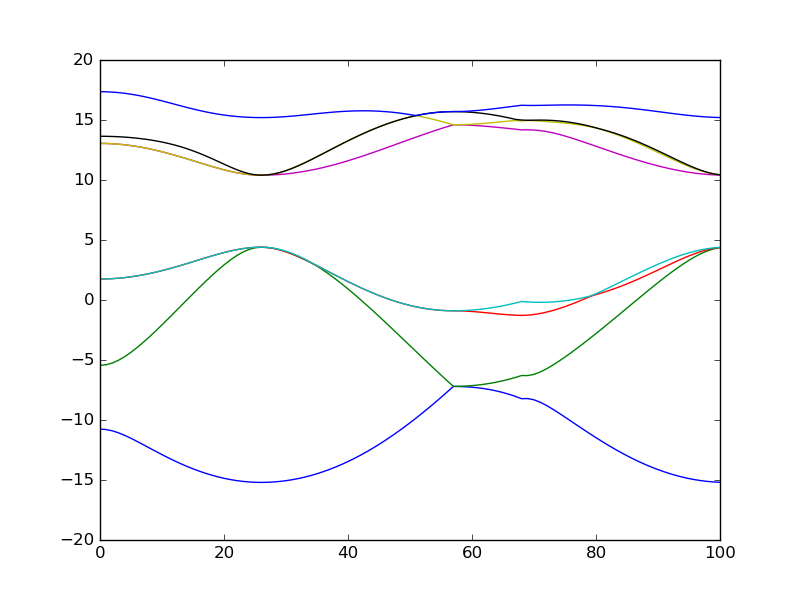
\includegraphics[width=\linewidth]{img/diamond_sp}
  \caption{Calculated band structure of diamond. \label{fig:tb_diamond}}
\end{figure}
\begin{figure} 
\begin{center}
  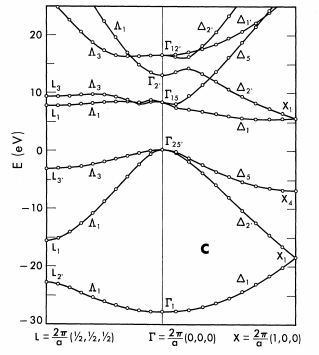
\includegraphics[width=0.5\linewidth]{img/diamond_exp_band_struct}
  \caption{Band structure of diamond (experiment). \label{fig:theory_diamond}}
\end{center}
\end{figure}  
